\section{Triality: present for 4+4, absent for 7+1}
\label{sec:triality}

Cartan discovered in 1925 that the rotation group of eight dimensions has a symmetry of order three,
\emph{triality}, that permutes its three inequivalent eight-dimensional representations---the vectors
$V_{\rm NG}$ and the two kinds of half-spinors $S^+_{\rm NG}$ and $S^-_{\rm NG}$---and he proved it by identifying all three
spaces with the octonions~\cite{Cartan1925,Baez2002}. In the language of Lie algebras, triality is an
\emph{outer} automorphism of $\mathfrak{so}(8)$: a map of the algebra onto itself that preserves
commutators but is not a conjugation by a rotation. Whether it survives on a spacetime of signature
$7+1$ or $4+4$ is a question about the \emph{real form} of the algebra, and the answers differ.

\emph{Local triality.} Let $\mathbb A_{\rm NG}$ be $\mathbb O_{\rm NG}$ or $\mathbb O'_{\rm NG}$ and
$\mathfrak{so}(N_{\rm NG})$ the Lie algebra of the linear maps $\mathsf m$ of the algebra that preserve its
norm infinitesimally, $\langle\mathsf m\mathsf x,\mathsf y\rangle_{\rm NG}+\langle\mathsf x,\mathsf m\mathsf y\rangle_{\rm NG}=0$:
$\mathfrak{so}(8)$ for the octonions, $\mathfrak{so}(4,4)$ for the split octonions. The principle of local
triality~\cite{Schafer1966} states that for every $\mathsf m_1$ in this algebra there is exactly one pair
$(\mathsf m_2,\mathsf m_3)$ in it with
\begin{equation}
\mathsf m_1(\mathsf x\mathsf y)=(\mathsf m_2\mathsf x)\mathsf y+\mathsf x(\mathsf m_3\mathsf y)\qquad\text{for all }\mathsf x,\mathsf y.
\label{eq:lt}
\end{equation}
For each of the 28 basis elements $\mathsf m_1$ the program writes Eq.~(\ref{eq:lt}) on all 64 pairs of
basis elements as 512 linear equations for the 56 coefficients of $\mathsf m_2$ and $\mathsf m_3$ and solves
them exactly: the system is consistent and its solution unique, for both algebras (check T-1). The
maps $T^{(2)}_{\rm NG}:\mathsf m_1\mapsto\mathsf m_2$ and $T^{(3)}_{\rm NG}:\mathsf m_1\mapsto\mathsf m_3$ preserve all
378 commutators of basis elements, are invertible, and are involutions (checks T-2, T-3).

\emph{They are outer.} A conjugation by a matrix does not change the characteristic polynomial. The
generator $\mathsf r_{01}$ of rotations in the plane of $\mathsf e_0$ and $\mathsf e_1$ (with
$\mathsf r_{01}\mathsf e_1=\mathsf e_0$, $\mathsf r_{01}\mathsf e_0=-\mathsf e_1$, and zero on the other six units) has
$\det(\lambda_{\rm NG}\mathsf 1_8-\mathsf r_{01})=\lambda_{\rm NG}^6(\lambda_{\rm NG}^2+1)$, the spectrum of a vector
representation (eigenvalues $\pm i$ and six zeros). Its images have
$\det(\lambda_{\rm NG}\mathsf 1_8-T^{(2)}_{\rm NG}\mathsf r_{01})=\det(\lambda_{\rm NG}\mathsf 1_8-T^{(3)}_{\rm NG}\mathsf r_{01})=
(\lambda_{\rm NG}^2+\tfrac14)^4$, the spectrum of a half-spinor representation (eigenvalues $\pm i/2$, four
times each), computed exactly (check T-4, Fig.~\ref{fig:triality}). With the conjugation
$\kappa_{\rm NG}:\mathsf x\mapsto\bar{\mathsf x}$, which is a reflection and induces the automorphism
$\mathrm{Ad}\,\kappa_{\rm NG}:\mathsf m\mapsto\kappa_{\rm NG}\mathsf m\kappa_{\rm NG}$, the composition
$\vartheta_{\rm NG}=T^{(2)}_{\rm NG}\circ\mathrm{Ad}\,\kappa_{\rm NG}$ has order three ($\vartheta_{\rm NG}^3=1\ne
\vartheta_{\rm NG}$), and $\mathrm{Ad}\,\kappa_{\rm NG}\,\vartheta_{\rm NG}\,\mathrm{Ad}\,\kappa_{\rm NG}=
\vartheta_{\rm NG}^{-1}$: these automorphisms generate the permutation group of three objects, the outer
automorphism group of $\mathfrak{so}(8)$ (check T-5). For the split octonions the program also confirms
that the images have exactly the spectrum of the half-spinor generators of the project: the two
$8\times8$ diagonal blocks of $\Sigma^{01}_{1644}=\tfrac14[\gamma^0_{1644},\gamma^1_{1644}]$, which act on
the real half-spinors $S^\pm_{\rm NG}$ of $4+4$, both have the characteristic polynomial
$(\lambda_{\rm NG}^2+\tfrac14)^4$ (check T-6).

\begin{figure}[t]
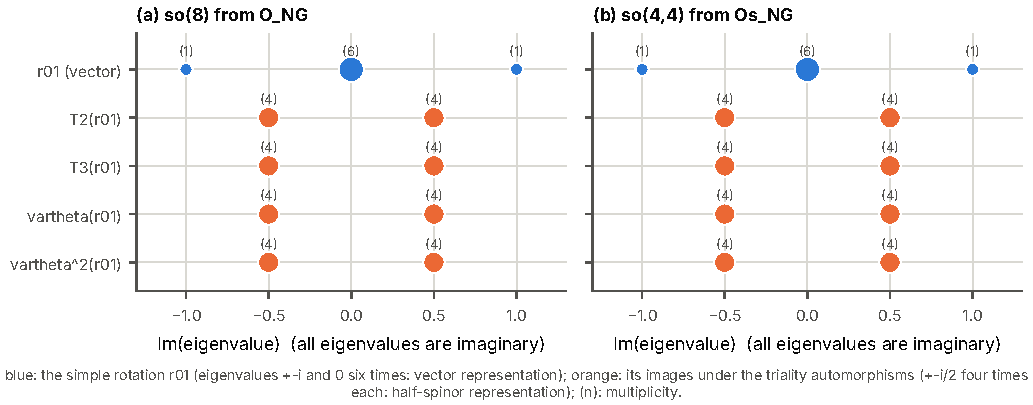
\includegraphics[width=\columnwidth]{../figures/fig_ng_triality.pdf}
\caption{Triality changes the spectrum of a rotation generator from that of a vector (blue: $\pm i$
and six zeros) to that of a half-spinor (orange: $\pm i/2$, four times each), for $\mathfrak{so}(8)$ (a)
and $\mathfrak{so}(4,4)$ (b). The numbers give multiplicities. Data:
\texttt{data/ng\_triality\_charpolys.csv} (exact characteristic polynomials).}
\label{fig:triality}
\end{figure}

\emph{Theorem 2 (no triality for $7+1$).} No automorphism of the Lorentz algebra
$\mathfrak{so}(7,1)$ maps its vector representation onto a half-spinor representation.
\emph{Proof.} (a) A real representation whose commuting matrices (its \emph{commutant}) form the
real numbers is of real type; one whose commutant is a copy of the complex numbers is of complex
type. Composing a representation with an automorphism does not change its matrices as a set, hence
not its commutant or its type. (b) The vector representation of $\mathfrak{so}(7,1)$ has commutant
$\mathbb R$ (check T-7d). (c) On the 16 real spinor components the commutant of the 28 generators
$\Sigma^{AB}_{1671}$ is spanned by $\mathsf 1_{16}$ and $\omega_{1671}=\gamma^0_{1671}\cdots
\gamma^7_{1671}$, and $\omega_{1671}^2=-\mathsf 1_{16}$ (check T-7b): the spinor representation is
irreducible over the real numbers and of complex type, so there is no real half-spinor representation
of dimension 8 at all; over the complex numbers the two half-spinors are complex conjugates of each
other. Hence no automorphism can map the vector representation (real type, dimension 8) onto a
half-spinor. $\square$

By contrast, on $4+4$ the commutant of the $\Sigma^{AB}_{1644}$ is spanned by $\mathsf 1_{16}$ and
$\omega_{1644}$ with $\omega_{1644}^2=+\mathsf 1_{16}$ (check T-7c): the spinors split into two real
half-spinors of dimension 8 (Majorana-Weyl spinors), and triality permutes $V_{\rm NG}$, $S^+_{\rm NG}$, $S^-_{\rm NG}$, all real.
A direct test agrees: for the boost $\mathsf m_1$ that mixes $\mathsf e_0$ with $\mathsf e_1$ in the metric
$\mathrm{Re}(\mathsf x^2)$ of $7+1$ (it maps $\mathsf e_0\mapsto\mathsf e_1$ and $\mathsf e_1\mapsto\mathsf e_0$),
Eq.~(\ref{eq:lt}) has no solution even with arbitrary $8\times8$ matrices $\mathsf m_2$, $\mathsf m_3$ (check
T-7a). Cartan's triality lives on the complex algebra $\mathfrak{so}(8,\mathbb C)$ and on those of its real
forms whose three eight-dimensional representations are real---the compact $\mathfrak{so}(8)$ and the split
$\mathfrak{so}(4,4)$; the octonions build the Dirac matrices of $7+1$ (Sec.~\ref{sec:octonions}), but
the order-three automorphism does not restrict to $\mathfrak{so}(7,1)$, which keeps only the reflection.
